\chapter{Resultados}
\label{chap:analiseresultados}
Inicialmente para criação da arquitetura especificada na seção \ref{chap:arquitetura}, criou-se o serviço de \textit{Command}, o qual é a porta de entrada entre a interface de usuário e a arquitetura, este serviço tem a função de receber os dados da interface (dispositivo embarcado), validá-los e inserir na fila de mensagens, a qual foi montada se utilizando o Kafka, é através deste micro serviço que um carro terá a sua sessão criada (\textit{Command Session}), informará dados sobre a localização (\textit{Command Track}), ou ainda informações de alerta (\textit{Command Warning}), para isso, como pode ser observado no apêndice \ref{ap:sessioncommand}, se tem as validações de campos para cada um dos modelos de dados, no caso das informações referentes a sessão se tem informações sobre a marca, modelo, placa e  proprietário, no modelo de dados de localização se tem o identificador da sessão, nível de combustível, latitude, longitude e velocidade, e no modelo de dados referentes a alertas o identificador da sessão e o alerta emitido pelo veículo. Todos estes dados são manipulados e recebidos no formato \textit{JavaScript Object Notation} (JSON) por questões de velocidade e uso de memória. Ainda no apêndice  \ref{ap:sessioncommand} é apresentado todos os comandos de envio para a fila do Kafka de cada um dos modelos de dados.

Seguindo a arquitetura, tornou-se necessário a configuração da fila de mensagens (Kafka), a qual tem a função de armazenar uma informação por um determinado tempo até que ele expire depois de um tempo pré configurado. Para isso utilizou-se imagens Docker vindas de repositórios oficiais, sendo necessário um contêiner com a imagem do Kafka Zookeeper, o qual é o sistema responsável por gerenciar os \textit{brokers} do Kafka, e outro contêiner com a imagem do Kafka Broker, no qual se tem os \textit{brokers} própriamente dito, cada um funcionando em um contêiner separado.

O próximo passo que se tem dentro da arquitetura é a criação do micro serviço \textit{Worker}, o qual tem a finalidade de ler dados da fila de mensagens e armazená-las nos bancos de dados, para isso este micro serviço foi criado em Clojure, contendo a conexão com o Kafka, além das conexões com os bancos de dados MongoDB e Datomic, o apêndice \ref{ap:sessionworker} mostra a retirada de dados da fila de mensagens e gravação dos dados nas duas bases de dados, de acordo com o tipo de informação contida na mensagem.

Por fim foram configurados os bancos de dados, os quais armazenam os dados vindos dos serviços de \textit{Workers} e os mantém para consultas instantâneas no caso do MongoDB, ou consultas históricas no caso do Datomic. Para os dois bancos de dados utilizou-se de imagens Docker oficiais com a base de dados armazenadas no \textit{host}, para que os dados fiquem disponíveis para todas as réplicas, fazendo a função de \textit{pipeline} entre os contêineres, mesmo quando estes sejam replicados.

Tendo os dados armazenados, para o processo de leitura destes dados criou-se o micro serviço \textit{Command Query} também em Clojure, o qual tem a função de ler os dados inseridos no MongoDB, sem passar pela fila de mensagens, diretamente ele realiza a função de busca no banco de dados de acordo com a informação requisitada, retornando para o usuário que requisitou a informação que passará a ser exibida na interface do usuário.

Todos os micro serviços  utilizados dentro da arquitetura apresentam-se encapsulados dentro de contêineres, estes porém, possuem a base inicial vinda de uma imagem Docker oficial, no caso destes micro serviços utilizou-se a imagem Java com \textit{Java SE Runtime Environment} (JRE) em sua versão 8, sendo assim, as alterações e configurações para o ambiente desejado se fizeram através do Dockerfile, que ao ser construído gera uma nova imagem com as alterações nele contidos, e para criação do contêiner basta especificar que a imagem a ser usada será esta nova imagem.

Tendo as imagens criadas, para facilitar o processo de instalação de toda a arquitetura no servidor desejado criou-se o arquivo Docker Compose, através dele são especificados os contêineres que serão instanciados, bem como as portas e variáveis de ambiente para cada micro serviço, é função  dele manter o funcionamento dos contêineres e reiniciá-los em caso de falha, através dele também foi possível maior facilidade quando necessário parar ou reiniciar algum serviço. Como mostrado no apêndice \ref{ap:dockercompose}, são criados os contêineres para os micro serviços tendo conexões para os bancos de dados e a fila de mensagens, desta forma no servidor em que é instalado a arquitetura é possível observar o  \textit{cluster} de contêineres funcionando, como apresentado na figura \ref{fig:dockerps}.

\begin{figure}[!h]
\caption{\label{fig:dockerps} Cluster de Contêineres}
\begin{center}
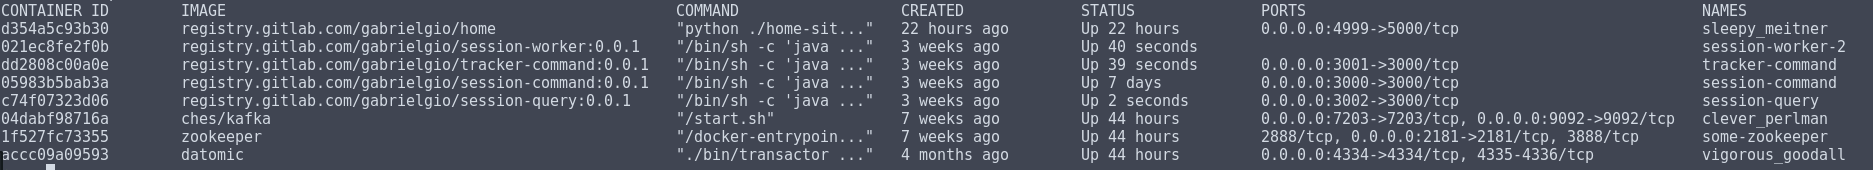
\includegraphics[scale=0.3]{dockerps}
\end{center}
%\legend{Fonte: \citeauthor{cqrs}, \citeyear{cqrs}} 
\end{figure}

Para verificação do fluxo de dados e validação da arquitetura criada, desenvolveu-se uma aplicação em Python, a qual apresenta uma interface para visualização dos veículos conectados a infraestrutura em tempo real, além das informações enviadas através destas conexões, se utilizando de \textit{sockets} para isso, tal aplicação se tornou útil para verificação das simulações que serão descritas na seção \ref{sec:testessistema}, pois através desta foi possível a visualização dos dados simulados de forma simples, como pode ser visto na figura \ref{fig:prototipo}.

\begin{figure}[!h]
\caption{\label{fig:prototipo} Visualização dos clientes}
\begin{center}
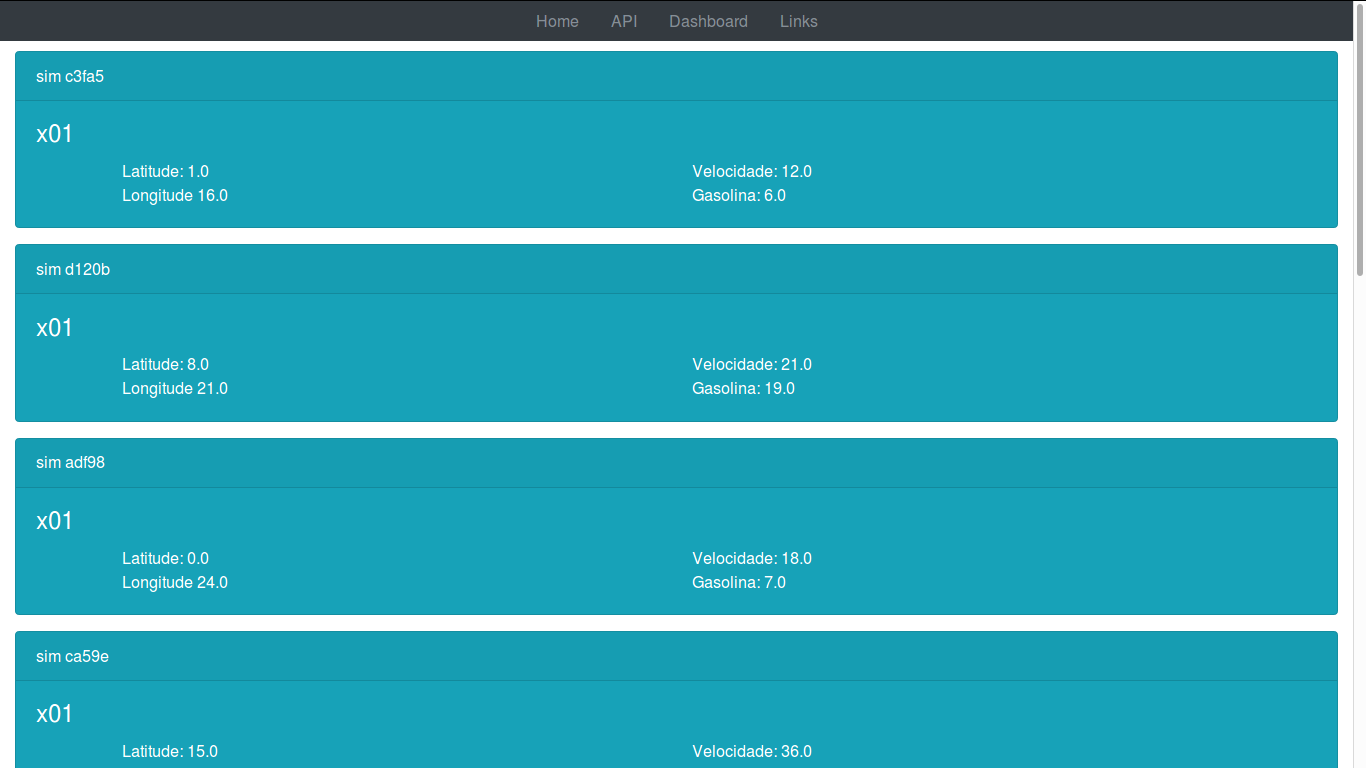
\includegraphics[scale=0.3]{prototipo}
\end{center}
%\legend{Fonte: \citeauthor{cqrs}, \citeyear{cqrs}} 
\end{figure}

\section{Testes de Sistema}
\label{sec:testessistema}
Para testes da arquitetura, realizou-se a instalação da mesma em um servidor no provedor de serviços \textit{Server as a Service} (SaaS) Azure, com uma máquina de 8 GB de memória e 2 núcleos de CPU, então para testes de carga sobre a arquitetura, bem como teste de integridade de dados mesmo sobre alta pressão, foi desenvolvido um \textit{Mockup}, cujo o conceito é simular funcionalidades do sistema para que estas possam ser testadas de forma independente, sendo assim, dentro desta arquitetura os objetos \textit{mock} foram os carros e unidades de emergência, os quais tiveram seu comportamento simulado via \textit{software}, a fim de validar o armazenamento e fluxo de dados na arquitetura.

O \textit{Mockup} realizou-se por meio de um micro serviço escrito em Clojure, apresentado no apêndice \ref{ap:mockveiculos}, o qual cria uma quantidade de conexões pré-estabelecidas com o micro serviço \textit{Session Command} e envia dados fictícios como a criação de uma sessão, localização e informações referentes a nível de combustível e alertas em cada conexão criada, destas informações, nível de combustível e campos texto na criação da sessão se fizeram de forma aleatória, já a latitude e longitude se fez de forma a apresentar rotas reais para que estes pudessem receber os alertas das unidades de emergência, como mostra no apêndice \ref{ap:mockveiculos}, sendo assim, foi possível obter os dados sobre consumo de memória e quantidade de requisições por segundo como apresentado na tabela \ref{tab:resultados}.

\section{Discussão de Resultados}
\label{sec:discussãoresultados}
Através dos resultados apresentados é possível verificar que a arquitetura se adéqua ao propósito do seu desenvolvimento, apresentando uma alta escalabilidade através das ferramentas empregadas e alta velocidade no processamento das requisições, algo que é crucial para o tipo de uso, em que informações devem ser entregues no menor tempo possível.

Com relação ao seu desenvolvimento ferramentas como Docker e Docker Compose provaram ser muito úteis quando o assunto é realizar \textit{deploy} de uma aplicação de forma rápida, diminuindo consideravelmente o tempo para instalação de todo o ambiente de produção.